\cleardoublepage
%\begin{refsection}
\chapter{Interference model of HIFI Band~1}
\label{sec:chapter4}


%#############################################################################
\section{Introduction}
The previous chapters describe a physically-based model that we created to predict the effect of interferences in coherent detectors.
This chapter compares our model to observational data from the HIFI instrument~\parencite{AA_518_L6}.
Our goal is to validate our model and to derive parameters several system parameters for the HIFI instrument that are only approximately known from its design and commissioning.

We choose to model HIFI Band~1.
Bands~1, 2 and 5 of HIFI have fewer optical elements than Bands~3, 4, 6 and 7, making them easier to model by reducing the number of free parameters.
Indeed, Bands~3, 4, 6 and 7 use rooftop mirrors to form Martin--Puplett interferometers in order to maximize the coupling of the mixer to the sky and the local oscillator at the same time.
In Bands~1, 2 and 5, the LO power is high enough and there is no need to maximize its coupling to the mixer, allowing for a simpler design with less side-effects.
The coupling of the LO to the mixer is very weak in Band~1, which means that the LO--mixer cavities produce almost no interference;
this reduces again the number of parameters.
\Textcite{risacher2011standingwaves} confirms that the LO--mixer ripples are not detected in Band~1.

In a typical observation, HIFI takes four measurements: one on the source of astronomical interest, one on a part of the sky devoid of emission, and one on the hot and cold internal calibration loads.
The integrations on the loads are used to calibrate the bandpass of the instrument.
Ideally, the loads are black bodies, which means that they are perfect absorbers.
In practice, the loads are not perfect black bodies but reflect a fraction of the incident electromagnetic waves.
Likewise, the mixer reflects a fraction of the incident wave.
These reflections create interferences that impact the bandpass calibration of the instrument and results in ripples on the spectra.




\begin{figure}
    \centering
    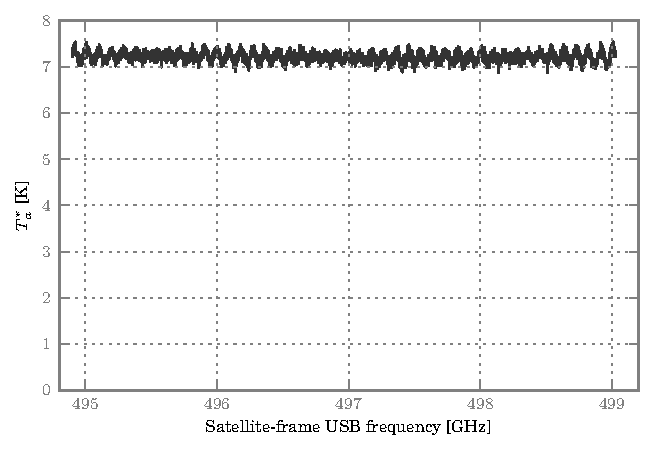
\includegraphics{mars_25_original}
    \caption{Observation of Mars by HIFI in Band~1 with the WBS-H showing a continuum modulated by ripples.
    Source: HSA, obsid 0x2fb00eb.}
    \label{fig:mars_25_original}
\end{figure}

The spectrum that we choose is shown in~\cref{fig:mars_25_original}.
It is an observation of the planet Mars recorded in Band~1 by the WBS-H backend, the wide-band spectrometer, horizontally polarized.
This spectrum shows a continuum modulated by ripples.
Atmospheric models of Mars predict a flat continuum, therefore we can attribute these ripples to an instrumental artifact that the calibration does not correct: interferences.
We choose this spectrum to validate our model because the ripples are relatively strong compared to the thermal noise present in the observation.
In this chapter, we use these ripples to derive the position of the loads, their reflection coefficient, and that of the mixer.

We begin the chapter with a brief description of the optics of HIFI Band~1.
Then we proceed to model the ripples in two steps.
First, we create a semi-analytic model, in which we model the ripples using ad-hoc perfect sinusoids.
This model gives us the periods of the ripples, which we can convert into approximate distances.
Second, we create a physically-based numerical model using the method detailed in~\cref{sec:chapter2}.


%#############################################################################
\FloatBarrier



\section{HIFI Band 1}
\Cref{fig:band1_layout} presents the optical layout of Band 1 of HIFI.
The signal from the local oscillator and the signal from the source are combined by a wire grid polarizer.
Two mixers detect the resulting beams.

Waves polarized in the plane of the page are called ``vertically polarized'' while waves polarized normally to the page are called ``horizontally polarized''.
The ``H~mixer'' detects horizontal waves, and the ``V~mixer'' detects vertical waves.

\begin{figure}
    \centering
    \footnotesize
    \input{band1_layout.pdf_tex}
    \caption{Layout of the optics of Band~1}
    \label{fig:band1_layout}
\end{figure}

Two wire grid polarizers ensure that the waves propagating toward the mixers are properly polarized for an optimal coupling to the mixer: they are noted ``H~grid'' and ``V~grid'' on the figure.
The wires of the H~grid are normal to the plane of the page and those of the V~grid lie in the plane of the page.
Grids are four-port devices (see~\cref{sec:wire_grid_polarizer}), two ports of each grids are dumped onto an absorber, getting rid of any unwanted polarization.

Three mirrors focus the beam from the grids into the horns of the mixers.

The signal from the sky is not polarized.
The thermal noise from the local oscillator and the calibration loads is not polarized either.
However, the useful signal of the local oscillator, that which pumps the mixers, is vertically polarized.

In Band~1, the local oscillator produces a beam whose power is much too high to properly pump the two mixers; most of the LO power needs to be dumped.
This is achieved by slightly rotating grid-0: its wires make an angle of~\SI{5.7}{\degree} with the plane of the page.
With that configuration, grid~0 sends most of the LO power down the H path, where it mostly goes through the H~grid into the dumps, and only a small fraction reaches the H~mixer.
The small fraction of LO power sent down the V~path by grid~0 is mostly reflected by the V~grid toward the V~mixer.
In the end, each mixer sees about~\SI{1}{\percent} of the LO power, the right amount of power to pump them optimally.

This very low coupling between the mixers and the local oscillator has an advantage: the LO--mixer cavities are very lossy and the interferences that they create are likely to be negligible.
In addition, the local oscillator itself is equipped with a~\SI{10}{\decibel} attenuator, which reduces interferences even more.
As a result, we expect that most of the ripples are caused by interferences in the cavities formed by the mixers and the calibration loads.
The coupling between the mixers and the local oscillator is greater in Bands~2 and 5; modeling them requires more parameters to account for this.





%#############################################################################
\FloatBarrier



\section{Analysis of the ripples}



%=============================================================================

\subsection{Smoothing}
In order to make the ripples more apparent, we smooth the original spectrum.
We do so by zeroing all power at periods shorter than a given threshold (\SI{40}{\mega\hertz} in our case).

\Cref{fig:mars_filtered} shows the result of that smoothing.
The original data is shown in black, the smoothed data in green and the residual in gray.

\begin{figure}
    \centering
    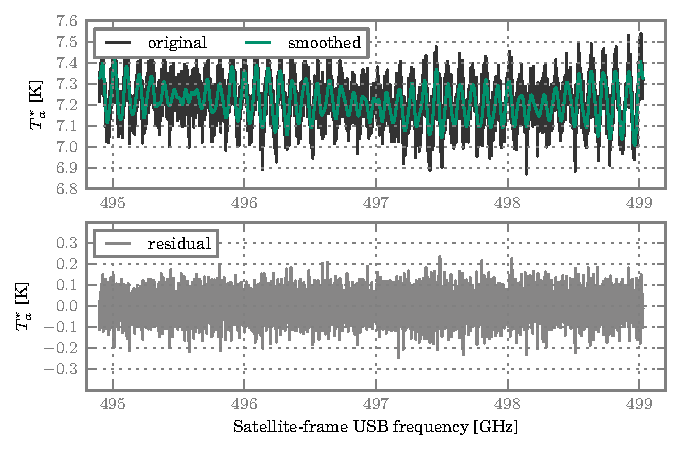
\includegraphics{mars_25_smoothed}
    \bigskip
    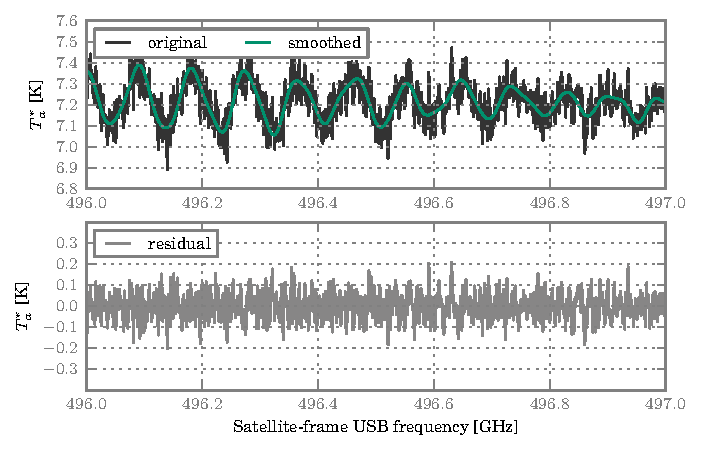
\includegraphics{mars_25_smoothed_zoom}
    \caption{
        Smoothing the spectrum of Mars separates the ripples from other sources of noise.
        Top: full spectrum, \SI{4}{\giga\hertz}-wide.
        Bottom: zoom on a \SI{1}{\giga\hertz}-wide region.
    }
    \label{fig:mars_filtered}
\end{figure}

The smoothed curve appears as a sinusoid wrapped in a sinusoidal envelope.
This ``beat'' pattern is typically produced when two sines of different but close periods are added together.
We are therefore expecting the contribution of two ripples, each coming from one cavity.
The period of the ripples, about~\SI{100}{\mega\hertz}, is compatible with the distance of about~\SI{1.5}{\meter} that separate the calibration loads from the mixer.
%\todo[inline]{Ref for the mixer--load distance, it's not easy to find, we mostly know it from previous standing waves analysis}
Indeed, the length~$d$ of a cavity and the period~$F$ of the ripple that it produces are linked by
the relation
\begin{equation}
    d = \frac{c}{2F}
    \label{eq:relation_length_period}
\end{equation}
in which $c$ is the speed of light in the medium, which we assume to be vacuum.
This equation is a rewrite of~\vref{eq:relation_length_period_nice}, in which the speed of light is made explicit.

An ideal spectrum for our purpose would combine a strong continuum, no spectral line, strong ripples and a low noise; but such spectra have little astronomical value and are therefore extremely rare, if at all present, in the HIFI database.
This spectrum shows very strong ripples which are helpful to constrain some parameters of our model.
Unfortunately, the thermal noise on top of these ripples is also very strong.
Indeed, the integration time of this observation is quite short: this observation was not designed to measure the continuum of Mars but to calibrate the pointing of the satellite.

%\begin{table}
%    \centering
%    \begin{tabular}{lc}
%        \toprule
%        spectrum & standard deviation [\si{\kelvin}]\\
%        \midrule
%        original & 0.101\\
%        smoothed & 0.080\\
%        residual & 0.061\\
%        \bottomrule
%    \end{tabular}
%    \caption{There is almost as much energy in the noise (residual) as in the ripples (smoothed).}
%    \label{tab:mars_filtered_stddev}
%\end{table}



%=============================================================================

\subsection{Fourier Transform}
Ripples are quasi-periodic features.
As such, they appear as peaks on a Fourier Transform.
\Cref{fig:mars_25_dft} shows the Discrete Fourier Transform of the spectrum of Mars.

\begin{figure}
    \centering
    \hfill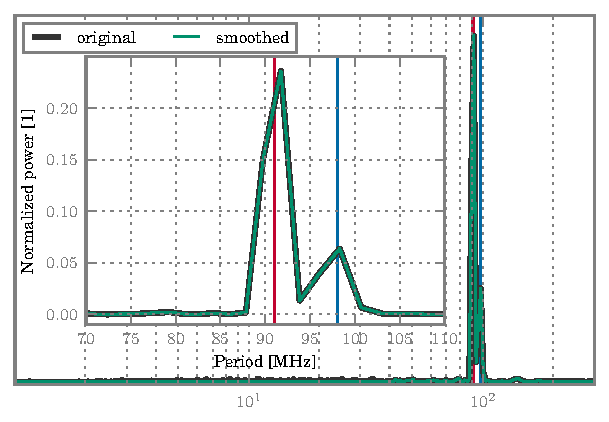
\includegraphics{mars_25_dft_lin}\\
    \hfill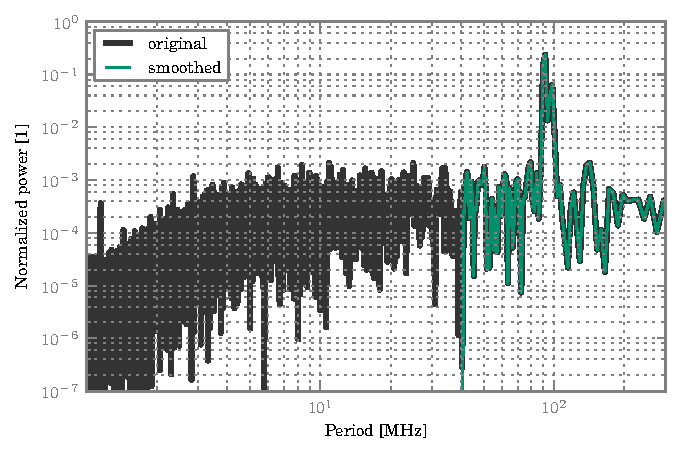
\includegraphics{mars_25_dft_log}
    \caption{
        Direct Fourier Transform of the original Mars spectrum (black) and its smoothed version (green).
        The inner plot zooms onto the two peaks.
        The vertical lines mark the approximate periods of the hot (red) and cold (blue) ripples.
        Top: linear vertical scale.
        Bottom: logarithmic vertical scale.
    }
    \label{fig:mars_25_dft}
\end{figure}

The horizontal axis of \cref{fig:mars_25_dft} represents the periods: short-period features are on the left, long-period features are on the right.
The continuum is not represented as it has an infinite period.
The vertical axis is either linear (top plot) or logarithmic (bottom plot).
In both cases, the vertical axis represents the power present at a given period.
Since our goal is to locate peaks, and not measure their power, the vertical axis has been normalized.

With its linear axis, the top plot shows that most of the power is concentrated into two peaks that are located at approximately~\SI{91}{\mega\hertz} and~\SI{98}{\mega\hertz}, marked by the red and blue vertical lines.
The resolution of the Fourier Transform is low at these periods, one would need spectra with a much broader frequency coverage to resolve these peaks.
The bottom plot is interesting because it shows no evidence of harmonics.
The fundamentals are located at~\SI{91}{\mega\hertz} and \SI{98}{\mega\hertz}, we could expect harmonics peaking at half these periods, and even weak harmonics would stand out on a logarithmic scale.
The lack of visible harmonics suggests that the cavities that create the ripple are very lossy (see~\cref{sec:fabry_gain}), unless the resolution of the DFT is too low.

These plots in the Fourier domain bring evidence that we can model the ripples as two perfect sinusoids.



%=============================================================================

\subsection{Perfect-sines model}
\label{sec:perfect_sines_model}
Examining the Direct Fourier Transform of the spectrum shows evidence of two sinusoidal ripples but offers only a very crude approximation of their period.

To determine the periods of the ripples more accurately, we model the smoothed spectrum with three components: a polynomial of degree 1 for the baseline and two sinusoidal functions.

The baseline is modeled with~$y=a(f-f_0)+b$ where
$f$ the frequency of the channel and
$f_0=\SI{496974750000}{\hertz}$ is the frequency in the middle of the spectrum.
Each ripple is modeled with~$y = C \cos(\phi) + S \sin(\phi)$ where
$\phi = 2 \pi f / F$ and $F$ is the period of the sine.

The model parameters are given in \cref{tab:two_sines_fit}.
This model gives us a much better estimate of the periods of the ripples than the one provided by the DFT.
\Cref{fig:mars_sine_fit} illustrates the differences between the smoothed spectrum of Mars and its model using perfect sines.


\begin{table}
% Cont result ['7.211908771679127', '-1.262493598126238e-11']
% Cont errors ['5.614822816527074e-05', '4.7109413498749796e-14']
    \centering
    \begin{tabularx}{\textwidth}{X c c}
        \toprule
            &
            slope $a$ [\si{\kelvin\per\hertz}]
            &
            average $b$ [\si{\kelvin}]
            \\
        \midrule
            baseline
            &
            $\num{-1.262e-11} \pm \num{4.7e-14}$
            &
            $\num{7.21191} \pm \num{5.6e-05}$
            \\
        \bottomrule
    \end{tabularx}
    \bigskip
% Hot  result ['-0.024374668042950198', '-0.084177761411197496', '90964727.019958138']
% Hot  error  ['0.032581863729936822', '0.0094248123566952492', '1025.6247261452409']
% Cold result ['-0.03334118353679541', '-0.039445727877105055', '97604192.684090942']
% Cold error  ['0.026008970168651415', '0.021974915562550285', '2011.3533923905459']
    \begin{tabularx}{\textwidth}{X c c c}
        \toprule
        ripple
        &
            $\cos$ amplitude $C$ [\si{\kelvin}]
        &
            $\sin$ amplitude $S$ [\si{\kelvin}]
        &
            period $F$ [\si{\hertz}]
        \\
        \midrule
        hot &
        $\num{-0.01965} \pm \num{0.00055}$ &
        $\num{ 0.08539} \pm \num{0.00013}$ &
        $\num{90964800} \pm \num{1000}$ \\
        cold &
        $\num{-0.03658} \pm \num{0.00032}$ &
        $\num{ 0.03645} \pm \num{0.00032}$ &
        $\num{97604400} \pm \num{2100}$\\
        \bottomrule
    \end{tabularx}
    \caption{
        Parameters modeling the baseline and the ripples of the smoothed spectrum of Mars with a polynomial and two sinusoids.
    }
    \label{tab:two_sines_fit}
\end{table}

\begin{figure}
    \centering
    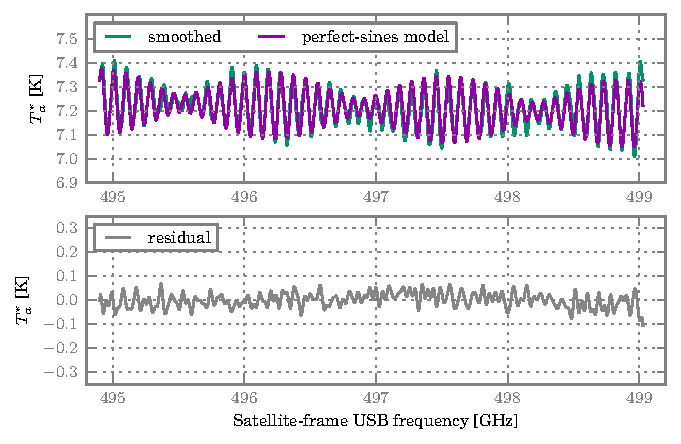
\includegraphics{mars_25_sine_fit}
    \caption{Model of the ripple using two sinusoids.}
    \label{fig:mars_sine_fit}
\end{figure}

Using~\cref{eq:relation_length_period} with $c=c_0$ (the speed of light in vacuum), we get our first estimate of the length of the cavities which we give in~\cref{tab:first_estimate_cavity_length}.
The mixer and the hot load are separated by~\SI{1.64}{\meter}, the mixer and the cold load by~\SI{1.53}{\meter}.
These are optical path lengths, not actual distances.
Assuming~$c=c_0$ is justified by the fact that the focal plane unit of HIFI is in vacuum.
However, this assumption suggests that there is only vacuum between the loads and the mixers, which we know is not the case since there are two grids and three mirrors in that optical path.
Furthermore, the surface of a load is a mathematical one: a load does not present a perfectly plane surface normal to the beam; we assume that the load behave as if it had an effective plane surface at a given effective distance.
For these two reasons, we expect that the optical path lengths that we just calculated differ somewhat from the actual distances between the mixers and the loads.

\begin{table}
    \centering
    \begin{tabular}{lcc}
        \toprule
        ripple &
        period [\si{\hertz}] &
        pathlength [\si{\meter}] \\
        \midrule
        hot  & $\num{90964800} \pm \num{1000}$ & $\num{1.64785} \pm \num{0.00004}$ \\
        cold & $\num{97604400} \pm \num{2100}$ & $\num{1.53575} \pm \num{0.00006}$ \\
        \bottomrule
    \end{tabular}
    \caption{First estimation of the distance between the mixer and the loads, from the
    period of the ripples.}
    \label{tab:first_estimate_cavity_length}
\end{table}





%#############################################################################
\FloatBarrier



\section{Interference modeling of HIFI Band 1}
We apply the method of~\cref{sec:chapter2} to model the optics of HIFI.
We rely on this model to predict the interferences in the mixer--load cavities.

The interference model alone can only predict the gains of the system for a given input.
In order to reproduce the spectrum of Mars, we need to apply these gains to an input power.


First, we describe how we must calibrate the output of our model to reproduce the spectrum of Mars.
Then, we present the configuration of networks that we use to model the optics of Band~1 and predict its gains.
Finally, we determine the powers, and therefore electric field amplitudes, that enter our system.



%=============================================================================

\subsection{Calibration equation}

The spectrum of Mars shown in~\cref{fig:mars_25_original} is the result of the standard HIFI calibration pipeline \parencite{hifiobserversmanual}.
This pipeline applies the reference subtraction and the bandpass calibration described in \textcite{ossenkopf2002intensity}.
It is summarized by the following equation:
\begin{equation}
    J_\text{src}(f)% - J_\text{ref}(f)
    = 
    \frac{
        c_\text{src}(f) - c_\text{ref}(f)
    }{
        c_\text{hot}(f) - c_\text{cold}(f)
    }
    (\eta_\text{hot} + \eta_\text{cold} - 1)
    (
        J_\text{hot}(f_\text{LO}) - J_\text{cold}(f_\text{LO})
    )
    \text{.}
    \label{eq:mars_calibration}
\end{equation}
$J_\text{src}(f)$ is the spectrum plotted on~\cref{fig:mars_25_original}, it would correspond to the power detected from Mars expressed as a Rayleigh--Jeans temperature if the calibration had properly removed the ripples.
The four values $c_\text{src}$, $c_\text{ref}$, $c_\text{hot}$ and $c_\text{cold}$ correspond to the output of the spectrometer expressed in its native arbitrary unit (``CCD counts'' for the WBS) for the four pointings done during the observation:
on Mars (``src''), on the blank sky (``ref'') and on the hot and cold calibration loads.
The two terms $\eta_\text{hot}$ and $\eta_\text{cold}$ are the power coupling efficiencies of the beam to the calibration loads.
Finally, $J_\text{hot}$ and $J_\text{cold}$ refer to the power emitted by the calibration loads, expressed as Rayleigh--Jeans temperatures.

For this observation,
$f_\text{LO} = \SI{490.97475}{\giga\hertz}$,
$\eta_\text{hot} = 0.959$,
$\eta_\text{cold} = 0.991$,
$T_\text{hot} = \SI{100.275}{\kelvin}$ and
$T_\text{cold} = \SI{13.134}{\kelvin}$.

The last two parameters, $T_\text{hot}$ and $T_\text{cold}$ are the physical temperatures of the calibration loads measured by thermometers during the observation.
Assuming that the loads are black bodies, their spectral radiance $B$ follow Planck's law.
\begin{equation}
    B
    =
    \frac{2 h f^3}{c^2} \frac{1}{e^{\frac{h f}{k_B T} - 1}}
    \label{eq:planck_law}
\end{equation}
Here, $T$ is the temperature of the load, $f$ is the frequency, $h$ is Planck's constant, $c$ is the speed of light in the propagation medium (vacuum for us) and $k_B$ is the Boltzmann constant.
We want to express their spectral radiance as Rayleigh--Jeans temperatures $J_\text{hot}$ and $J_\text{cold}$.
We do this by solving Rayleigh--Jeans' law for $J$.
\begin{equation}
    B
    =
    \frac{2 f_\text{LO}^2 k_B}{c^2}J
    \label{eq:rayleigh_jeans_law}
\end{equation}
The results are $J_\text{hot} = \SI{88.95}{\kelvin}$ and $J_\text{cold} = \SI{4.70}{\kelvin}$.
We must remember that HIFI is a double-sideband instrument: each channel of the spectrum contains a contribution from both sidebands.
When looking at a continuum source at a temperature $J$, HIFI receives $J$ in each sideband for a total of $2J$.
To compensate, the scaling factor $J_\text{hot} - J_\text{cold}$ must be multiplied by 2.
This is equivalent to having $J_\text{hot} = \SI{177.90}{\kelvin}$ and $J_\text{cold}=\SI{9.40}{\kelvin}$.


Rayleigh--Jeans' law is an approximation of Planck's law for low frequencies and/or high temperatures.
The difference between $T_\text{hot}$ and $J_\text{hot}$ and between $T_\text{cold}$ and $J_\text{cold}$ illustrates that this approximation is poor in the range of powers and frequencies at which HIFI operates.
Nevertheless, it is customary for radioastronomers to express powers as Rayleigh--Jeans temperatures.

Since our goal is to reproduce a real observation of Mars with our model of the optics of HIFI Band~1, we use the same equation and the same parameters to calibrate our model.
Our model must provide $c_\text{src}$, $c_\text{ref}$, $c_\text{hot}$ and $c_\text{cold}$.
This is the subject of the next sections.



%=============================================================================

\subsection{IF chain}
The Intermediate Frequency (IF) chain processes the signal output by the mixer.
It consists in amplifiers, filters, and eventually a detector.
In our case, the detector is a pixel of the CCD of the WBS.
The output $c$ of the detector is an affine function of the power of its input $P_\text{detector input}$:
\begin{equation}
    c = G_\text{detector} \; P_\text{detector input} + z
\end{equation}
in which $G$ converts the unit from power to CCD count, and $z$ is an arbitrary constant.
The subtractions and the division in the calibration equation remove $G$ and $z$ from our concern.
\begin{equation}
    \frac{
        c_\text{src} - c_\text{ref}
    }{
        c_\text{hot} - c_\text{cold}
    }
    =
    \frac{
        P_\text{detector input, src} - P_\text{detector input, ref}
    }{
        P_\text{detector input, hot} - P_\text{detector input, cold}
    }
\end{equation}

Each power $P$ in the previous equation is proportional to the square of the amplitude of the electric field.
That coefficient of proportionality also disappears during the division.
\begin{equation}
    \frac{
        c_\text{src} - c_\text{ref}
    }{
        c_\text{hot} - c_\text{cold}
    }
    =
    \frac{
        \abs{\cp{e}_\text{detector input, src}}^2
        -
        \abs{\cp{e}_\text{detector input, ref}}^2
    }{
        \abs{\cp{e}_\text{detector input, hot}}^2
        -
        \abs{\cp{e}_\text{detector input, cold}}^2
    }
\end{equation}

Finally, the electric field at the input of the detector is proportional to the electric field at the output of the mixer:
$\cp{e}_\text{detector input} = \cp{g}_\text{IF chain} \cp{e}_\text{mixer output}$.
The division removes once again the common factor~$\abs{\cp{g}_\text{IF chain}}^2$.
\begin{equation}
    \frac{
        c_\text{src} - c_\text{ref}
    }{
        c_\text{hot} - c_\text{cold}
    }
    =
    \frac{
        \abs{\cp{e}_\text{mixer output, src}}^2
        -
        \abs{\cp{e}_\text{mixer output, ref}}^2
    }{
        \abs{\cp{e}_\text{mixer output, hot}}^2
        -
        \abs{\cp{e}_\text{mixer output, cold}}^2
    }
\end{equation}
In other words, we can completely ignore the IF chain.



%=============================================================================

\subsection{Mixing}
Although mixers are non-linear devices, their useful output phasor is proportional to their input phasor in the case of small signals.
\begin{equation}
    \begin{aligned}
    \cp{e}_\text{mixer output}
    &=
    \cp{g}_\text{mixer, LSB} \;
    \cp{e}_\text{mixer input, LSB} \\
    &+
    \cp{g}_\text{mixer, USB} \;
    \cp{e}_\text{mixer input, USB}
    \end{aligned}
\end{equation}
The frequency of the input phasors are $f_\text{LSB}$ and $f_\text{USB}$.
The frequency of the output phasor is $f_\text{IF}$.
The gain $\cp{g}_\text{mixer}$ is intrinsic to the mixer, it may depend on the frequency and be different for the LSB and USB frequency.

As this equation shows, mixers are coherent devices: they operate in field, not in power.
Although correct at any instant $t$, this equation cannot be applied to our situation.
Indeed, HIFI spectra are integrated over several seconds, which is orders of magnitude above the coherence time of the LSB and USB signals.
The LSB and USB signals are both coherent on their own, but they are not correlated with each other for that long: they are not phase-locked to each other.
The proper way of combining the contributions of the LSB and USB signals is in power:
\begin{equation}
    \abs{\cp{e}_\text{mixer output}}^2
    =
    \abs{\cp{e}_\text{mixer output, LSB}}^2
    +
    \abs{\cp{e}_\text{mixer output, USB}}^2
\end{equation}
with
\begin{align}
    \cp{e}_\text{mixer output, LSB}
    &=
    \cp{g}_\text{mixer, LSB}
    \;
    \cp{e}_\text{mixer input, LSB}
    \\
    \cp{e}_\text{mixer output, USB}
    &=
    \cp{g}_\text{mixer, USB}
    \;
    \cp{e}_\text{mixer input, USB}
    \text{.}
\end{align}

The standard HIFI pipeline assumes that the gain is the same for both sidebands:
$\cp{g}_\text{mixer, LSB} = \cp{g}_\text{mixer, USB} = \cp{g}_\text{mixer}$.
We make the same assumption in our model.
The resulting term $\abs{\cp{g}_\text{mixer}}^2$ disappears during the bandpass calibration.
With the subscript ``mi'' standing for ``mixer input'', we get the following equality.
\begin{gather}
    \frac{
        c_\text{src} - c_\text{ref}
    }{
        c_\text{hot} - c_\text{cold}
    }\notag
    =
    \\
    \frac{
        \left(
            \abs{\cp{e}_\text{mi, LSB, src}}^2
            +
            \abs{\cp{e}_\text{mi, USB, src}}^2
        \right)
        -
        \left(
            \abs{\cp{e}_\text{mi, LSB, ref}}^2
            +
            \abs{\cp{e}_\text{mi, USB, ref}}^2
        \right)
    }{
        \left(
            \abs{\cp{e}_\text{mi, LSB, hot}}^2
            +
            \abs{\cp{e}_\text{mi, USB, hot}}^2
        \right)
        -
        \left(
            \abs{\cp{e}_\text{mi, LSB, cold}}^2
            +
            \abs{\cp{e}_\text{mi, USB, cold}}^2
        \right)
    }
\end{gather}

We must compute eight mixer input spectra: one per pointing and per sideband.
Each spectrum is the product of the optical gain by the input power.



%=============================================================================

\subsection{Optical gains}
We model the optics of HIFI Band~1 with the networks shown in~\cref{fig:band1_networks}.
Each optical element is modeled with a $n$-port network which is represented numerically by a scattering matrix.
Using the technique that we describe in~\cref{sec:chapter2},
we solve the output of the system for each channel, for different parameters and for all the relevant sources of power.
\begin{figure}
    \centering
    \footnotesize
    \input{band1_networks.pdf_tex}
    \caption{Networks of band 1.}
    \label{fig:band1_networks}
\end{figure}

The white rectangles of~\cref{fig:band1_networks} represent distances between the other networks.
\Cref{tab:known_distances} lists the known distances.
The unknown distances, which we are trying to determine, are the distances between grid~0 and the surface of the calibration loads: the two white rectangles on the left of the chopper.

\begin{table}
    \centering
    \begin{tabular}{ll}
        \toprule
        distance network     & length [\si{\meter}] \\
        \midrule
        grid 0 -- H grid     & \num{0.040}   \\
        grid 0 -- V grid     & \num{0.040}   \\
        H grid -- H mixer    & \num{0.204}   \\
        V grid -- V mixer    & \num{0.204}   \\
        grid 0 -- attenuator & \num{0.74585} \\
        attenuator -- LO     & \num{0.57361} \\
        \bottomrule
    \end{tabular}
    \caption{
        Known distances between the optical elements of HIFI Band~1.
        Source: Willem Jellema, private communication.
    }
    \label{tab:known_distances}
\end{table}

In HIFI, the chopper is an actuated mirror that directs the beam of the telescope toward the sky or the calibration loads.
In our model, we represent it with a network whose transmission coefficient equals either 1 or 0 so that it connects one and only one source to grid~0.

The reflection on the loads and the mixers is a combination of several reflections on different points of the loads.
We assume that the overall reflection is equivalent to a single effective reflection on an effective mathematical surface normal to the direction of propagation of the beam (see~\cref{sec:gray_body}).
Each load has two unknown parameters: a complex reflection coefficient and the position of its effective surface.

The parameters of the other networks used in our model are listed in~\cref{tab:network_parameters}.
All these values are estimates that we consider reasonable.

\begin{table}
    \centering
    \begin{tabular}{lr}
        \toprule
        grid wire radius                          & \SI{1}{\micro\meter} \\
        grid wire spacing (axis to axis)          & \SI{4}{\micro\meter} \\
        grid wire conductivity                    & \SI{1e7}{\siemens\per\meter}   \\
        LO reflection coefficient                 & $-\sqrt{0.05}$       \\
        mixer reflection coefficient, co-pol      & $-\sqrt{0.05}$       \\
        mixer reflection coefficient, cross-pol   & $-1$       \\
        mixer transmission coefficient, co-pol    & $\sqrt{0.95}$       \\
        mixer transmission coefficient, cross-pol & $0$       \\
        attenuator gain                           & \SI{-10}{\decibel}   \\
        coupling coefficient to hot load          & $\sqrt{0.959}$       \\
        coupling coefficient to cold load         & $\sqrt{0.991}$       \\
        \bottomrule
    \end{tabular}
    \caption{Network parameters used to model HIFI Band~1.}
    \label{tab:network_parameters}
\end{table}

The reflection coefficient of the local oscillator barely matters, as we have established earlier that the cavities involving the local oscillator are too lossy to produce measurable ripples.
We set it to reflect~\SI{5}{\percent} of the incoming power but experimentation with the model confirms that its effect is negligible: the model is barely insensitive to the value of this parameter; the reflections from the loads dominate by orders of magnitude.

The rectangular horn of the mixer is designed to couple one polarization (called ``co-pol'') and reflect the other (called ``cross-pol'').
This is why we set the cross-pol reflection coefficient to~\SI{100}{\percent}.
We begin our model by assuming a co-pol reflection of~\SI{5}{\percent} in power.
Later in this chapter, we free this parameter and let a fitting algorithm determine its value.
The transmission coefficient of the mixer represents the fraction of the electric field that the mixer actually detects and can down-convert to the intermediate frequency~(IF).



%=============================================================================

\subsection{Input powers}
The four inputs are Mars, a portion of blank sky, the hot load and the cold load.
The local oscillator is also an input (via its~\SI{120}{\kelvin} thermal noise) that is present in each pointing.

We assume that all the sources emit according to Planck's law.
For sources that are not black but gray bodies (such as the calibration loads), our optical model performs the appropriate attenuation automatically (see the gray body surfaces on~\cref{fig:band1_networks}).

We know the physical temperatures of the hot and cold loads:
\SI{100.275}{\kelvin} and \SI{13.134}{\kelvin}.
The power originating from Mars that enters our optics corresponds to a Rayleigh--Jeans temperature is about~\SI{7.2}{\kelvin} (average of the continuum), which translates into a physical temperature of \SI{11.8}{\kelvin}.
We set the local oscillator and the blank sky temperatures to zero.

Setting the LO temperature to~\SI{0}{\kelvin} is justified by the very high losses of the LO--mixer cavities.
Experiments with the model show that setting it to a more realistic~\SI{120}{\kelvin} has no significant influence on the predictions of the model.
Ignoring the LO completely speeds up the calculations.

Setting the blank sky temperature to~\SI{0}{\kelvin} is justified by the $T_a^*$ scale of the original spectrum.
A more correct treatment would require to know the extension of Mars and its position inside the telescope beam.
This is not required because the spectrum of Mars that we are trying to reproduce has its temperature axis in $T_a^*$: it ignores pointing and extension and assumes that Mars is a point source in the middle of the beam.
As a result, the background radiation completely disappears in the power subtraction $P_\text{src}-P_\text{ref}$ and we can ignore it.

Our optical model does not operate on powers but on electric fields.
The SI units of these electric fields is \si{\volt\per\meter}.
The corresponding SI unit for power is a power density in \si{\watt\per\meter\squared}.
The power density is proportional to the square of the absolute value of the field amplitude.
That coefficient of proportionality disappears during the bandpass calibration and we do not need to know it.
Planck's law does not give a power density but a spectral radiance, expressed in
\si{\watt\per\meter\squared\per\steradian\per\hertz}.
The coefficient of proportionality in~\si{\per\steradian\per\hertz} that relates the spectral radiance and the power density also vanishes during the bandpass calibration, we do not have to calculate it either.
For our practical purpose, intensities equal the square root of powers.

Finally, all our sources are thermal noise.
As such, their radiation is unpolarized.
\Cref{sec:jones_unpolarized} describes how to treat unpolarized sources:
they are decomposed into two polarized sources of opposite polarizations, and their individual contributions are added in power.

We have defined all the steps that we take to model our spectrum of Mars.
In the next section, we confront that model to the original data taken by HIFI.





%#############################################################################
\FloatBarrier



\section{Hot and cold ripple fit}

Fitting periodic pattern is notoriously problematic:
when the objective function is a~$\chi^2$, then is has many local extrema in which the fitter can get stuck.
To avoid that problem, we fit our model in two steps.
\begin{enumerate}
    \item match the period and the phase of the ripples, and
    \item match the rest.
\end{enumerate}
We have two ripples: one caused by the hot load and one by the cold load.
The period and the phase of each ripple depend on the length of the cavity and the argument of the reflection coefficient of the load.
In this section, we fit the two mixer--load distances and the argument of the reflection coefficient.

We use the word ``argument'' instead of ``phase'' for the reflection coefficient because we already use the word ``phase'' for the phase of the sinusoid of the ripple.
The reflection coefficient is a complex number with a magnitude and an argument, we are fitting this argument.

Fitting two ripples at once can be difficult but we do not have to do it:
\cref{sec:perfect_sines_model} gives us a perfect-sine model for each ripple, independently of the other.
This allows us to fit two independent interference models, one for the hot and one for the cold ripple.
During the fits, we normalize the ripples predicted by the interference models.
Indeed, the folding step required by the mixing process adds the lower and upper sideband ripples together, which can be constructive or destructive, resulting in highly-variable amplitudes that mislead the fitters.
At this stage, we are interested only in the period and the phase, so we normalize the ripples.

\Cref{fig:mars_interf_stages_cold} shows different stages of the interference modeling of the cold ripple.
The top plot presents the gain of the modeled optical system;
it oscillates between \SI{80}{\percent} and almost \SI{100}{\percent}.
The second plot shows the optical gain multiplied by the actual power emitted by the cold black body: this is the power that couples to the mixer;
the slope results from a combination of Planck's law and Rayleigh--Jeans' law.
The third plot shows the effect of the mixer folding the spectrum;
this spectrum is the one that we compare to the perfect-sine model.
Finally, the bottom plot shows the sideband radio defined as $G_\text{USB}/(G_\text{LSB}+G_\text{USB})$;
channels that are USB-dominated have a sideband ratio greater than~\num{0.5}.

\begin{figure}
    \centering
    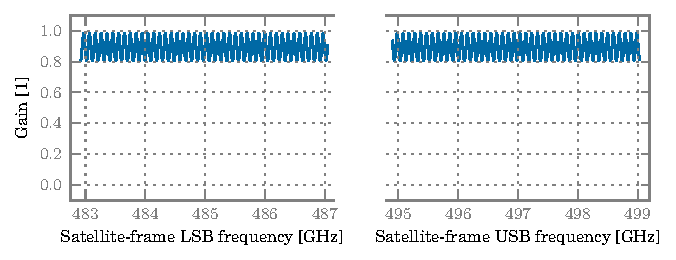
\includegraphics{mars_25_interf_dsb_gain_cold}
    \vspace{-1.1em}
    \caption*{Gain: what the mixer detects if the cold load emits a power of~1.}
    \medskip
    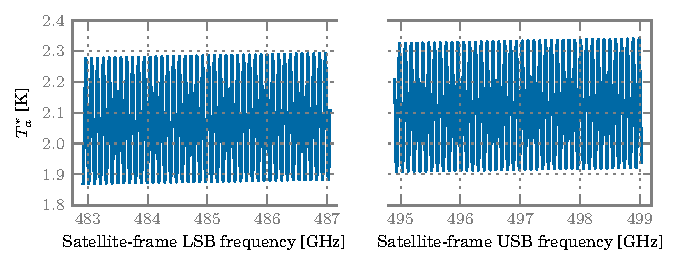
\includegraphics{mars_25_interf_dsb_temp_cold}
    \vspace{-1.1em}
    \caption*{Cold load power seen by the mixer before being folded.}
    \medskip
    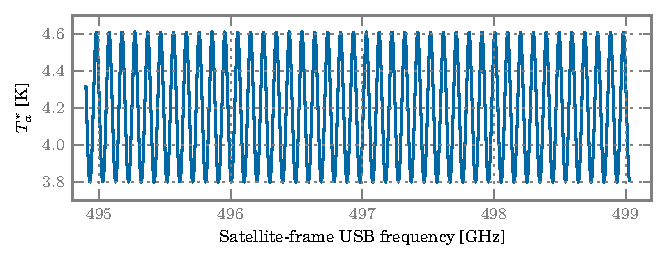
\includegraphics{mars_25_interf_fld_temp_cold}
    \vspace{-1.1em}
    \caption*{Cold load power seen by the mixer after being folded.}
    \medskip
    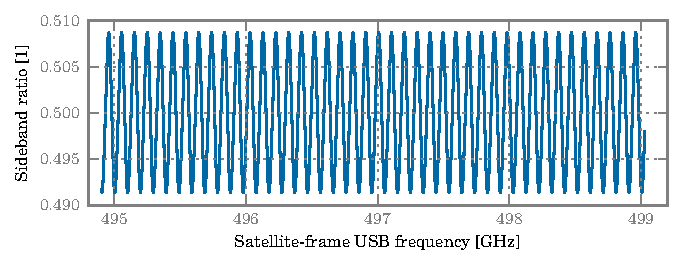
\includegraphics{mars_25_interf_sbr_cold}
    \vspace{-1.1em}
    \caption*{Sideband ratio: USB gain / (LSB gain + USB gain).}
    \caption{Three stages of the interference modeling for the cold load, and the sideband ratio.}
    \label{fig:mars_interf_stages_cold}
\end{figure}


\Cref{tab:interf_vs_perfectsine} lists the parameters of the interference model that best reproduce the perfect-sine model of the hot and the cold load.
The corresponding ripples are shown in~\cref{fig:mars_25_interf_distance_fit_cold,fig:mars_25_interf_distance_fit_hot}.
The vertical axis is arbitrary because the ripples are normalized.
Neither the hot and cold best interference models match the perfect-sine model perfectly.
This is due to the fact that some combinations of distance and argument produce ripples that do not approximate simple sines, as shown in~\cref{fig:mars_25_interf_distance_fit_cold_poor}.
\begin{table}
    % HOT
    % ## Distance param 1.6491521148703148
    % ## Distance error 8.5017794640728818e-05
    % ## Angle param 4.1068006437048581
    % ## Angle error 0.08755492869280726
    % X2 = 0.0085045429515
    % COLD
    % ## Distance param 1.5349642234206082
    % ## Distance error 6.4163290218112999e-05
    % ## Angle param 4.1915111156985274
    % ## Angle error 0.068293124275238634
    % X2 = 0.00289102399052
    \centering
    \begin{tabular}{l c c}
        \toprule
            load
            &
            distance [\si{\meter}]
            &
            argument [\si{\radian}] \\
        \midrule
            hot  & $\num{1.64915} \pm \num{8.5e-5}$    &    $\num{4.11} \pm \num{0.08}$ \\
            cold & $\num{1.53496} \pm \num{6.4e-5}$    &    $\num{4.19} \pm \num{0.06}$ \\
        \bottomrule
    \end{tabular}
    \caption{Parameters that make the interference model of the hot and cold spectra fit their perfect-sine model.}
    \label{tab:interf_vs_perfectsine}
\end{table}

\begin{figure}
    \centering
    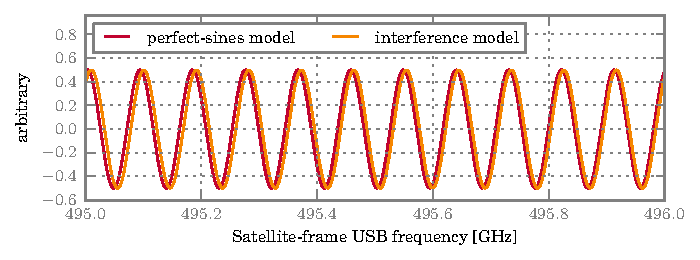
\includegraphics{mars_25_interf_distance_fit_hot}
    \caption{Best fit of the hot ripple.}
    \label{fig:mars_25_interf_distance_fit_hot}
\end{figure}
\begin{figure}
    \centering
    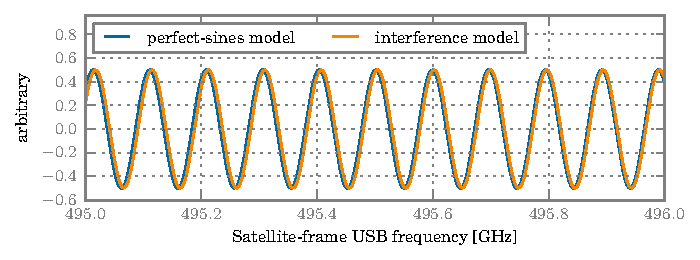
\includegraphics{mars_25_interf_distance_fit_cold}
    \caption{Best fit of the cold ripple.}
    \label{fig:mars_25_interf_distance_fit_cold}
\end{figure}
\begin{figure}
    \centering
    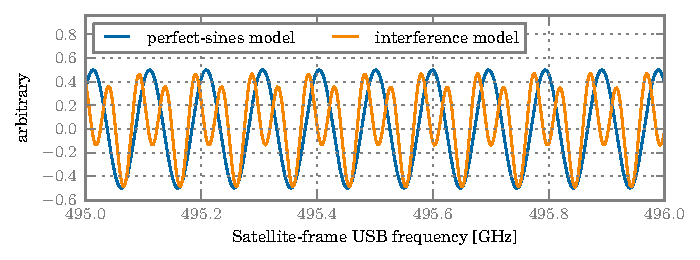
\includegraphics{mars_25_interf_distance_fit_cold_poor}
    \caption{Some narrow ranges of the argument of the reflection coefficient produce complex ripples that prevent a better fit.}
    \label{fig:mars_25_interf_distance_fit_cold_poor}
\end{figure}

We have compared one model to another in order to determine the mixer--load distances
and the argument of the reflection coefficient of the loads.
This gives us a very good first-guess to seed a fit that compares our complete interference model to the real data from Mars.





%#############################################################################
\FloatBarrier



\section{Full model fit}
The analysis done in the previous section gives us very good first-guesses for the mixer--load distances and the argument of the reflection coefficient of the two loads.
In this section, we compare our interference model to the real Mars data.

The free parameters are
\begin{itemize}
    \item the hot reflection coefficient, magnitude,
    \item the hot reflection coefficient, argument,
    \item the cold reflection coefficient, magnitude,
    \item the cold reflection coefficient, argument,
    \item the distance between the hot surface and the H mixer,
    \item the distance between the cold surface and the H mixer,
    \item and the physical temperature of Mars.
\end{itemize}

The interference model is compared to the smoothed version of the Mars spectrum, from which the linear trend (first-order polynomial fitted in~\cref{sec:perfect_sines_model}) is removed.
We remove the linear trend because our interference model does not predict it, it may be astronomical and not instrumental in nature.
Without a better model of Mars, we need to leave this trend out.

The result is shown in~\cref{fig:mars_25_interf_smoothed_vs_interf}.
The model parameters for this optimal solutions are listed in~\cref{tab:mars_full_model} for two cases:
in the first case, the coefficient of reflection of the mixer is fixed;
in the second case, it is a free parameter.

The uncertainties given in this table are very conservative estimates:
They are calculated assuming that their probability distribution is Gaussian, which obviously cannot be true for reflection coefficients that must reside inside the complex disk of radius~1.
We include them for the sake of disclosure, but a much better measurement of these uncertainties could be given by Bayesian analysis or Monte Carlo simulations.

\begin{figure}
    \centering
    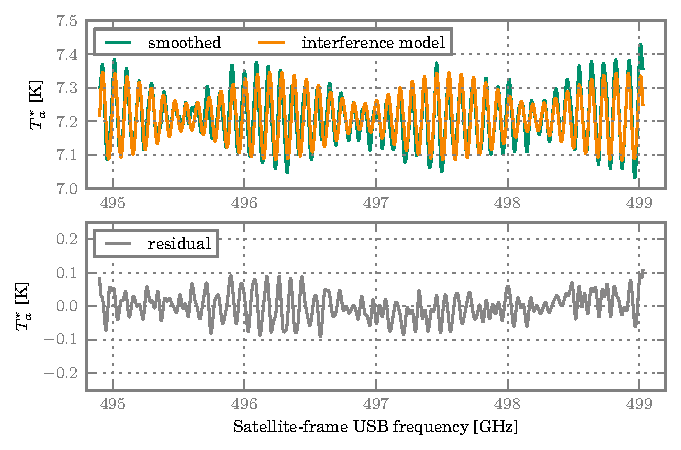
\includegraphics{mars_25_interf_smoothed_vs_interf}
    \caption{Best reproduction of the spectrum of Mars with our interference model.}
    \label{fig:mars_25_interf_smoothed_vs_interf}
\end{figure}

\begin{table}
    % 1.6480265532364544 +/-0.0012526911025520437
    % 1.5339021240876065 +/-0.0010667862540373438
    % 0.037896590464644483 +/-0.23324988755084228
    % 19.392660220711125 +/-31.097964720905996      0.5431042991723657
    % 0.3042926590794563 +/-0.75312073096021415
    % 24.807068124703694 +/-22.943509146023409      2.815919549575141
    % 11.725143032389045 +/-0.15502956205003632
    % STDDEV residual: 0.0380157531167
    \centering
    \begin{tabular}{l r@{}c@{}l r@{}c@{}l l}
        \toprule
        parameter &
        \multicolumn{3}{c}{value} &
        \multicolumn{3}{c}{uncertainty} & unit\\
        \midrule
            hot distance                                 &  1&.&6480  &  0&.&0012 & [\si{\meter}]  \\
            cold distance                                &  1&.&5339  &  0&.&0011 & [\si{\meter}]  \\
            hot reflection coefficient, magnitude        &  0&.&0379  &  0&.&23   & [1]            \\
            hot reflection coefficient, argument         &  0&.&5431  & 31& &     & [\si{\radian}] \\
            cold reflection coefficient, magnitude       &  0&.&3043  &  0&.&75   & [1]            \\
            cold reflection coefficient, argument        &  2&.&8159  & 23& &     & [\si{\radian}] \\
            mars temperature                             & 11&.&72    &  0&.&15   & [\si{\kelvin}] \\
        \bottomrule
    \end{tabular}
    \caption*{Case 1: The magnitude of the reflection coefficient of the mixer is fixed at~$-\sqrt{0.05}$.}
    \bigskip
    \begin{tabular}{l r@{}c@{}l r@{}c@{}l l}
        \toprule
        parameter &
        \multicolumn{3}{c}{value} &
        \multicolumn{3}{c}{uncertainty} & unit\\
        \midrule
            hot distance                                 &  1&.&6480 &  0&.&0012 & [\si{\meter}]  \\
            cold distance                                &  1&.&5339 &  0&.&0011 & [\si{\meter}]  \\
            hot reflection coefficient, magnitude        &  0&.&0442 &  0&.&34   & [1]            \\
            hot reflection coefficient, argument         &  0&.&55   & 31& &     & [\si{\radian}] \\
            cold reflection coefficient, magnitude       &  0&.&7033 &  3&.&07   & [1]            \\
            cold reflection coefficient, argument        &  2&.&40   & 21& &     & [\si{\radian}] \\
            mixer reflection, magnitude                  & -0&.&19   &  1&.&0    & [1]            \\
            mars temperature                             & 11&.&84   &  1&.&32   & [\si{\kelvin}] \\
        \bottomrule
    \end{tabular}
    \caption*{Case 2: The magnitude of the reflection coefficient of the mixer is free.}
    \caption{Interference model parameters that best reproduce the real Mars data.}
    \label{tab:mars_full_model}
\end{table}



%#############################################################################
\FloatBarrier



\section{Discussion}

Although the model seems to fit the data quite well in~\cref{fig:mars_25_interf_smoothed_vs_interf}, the residual shows strong sinusoidal features.
These are due to small mismatches in amplitude or in phase.
This model is not good enough to make quantitative predictions of the ripples, but its qualitative predictions are satisfactory.

The spectrum of Mars with which we have worked so far is part of a series of spectra taken with different pointings.
\Cref{fig:mars_24_interf_smoothed_vs_interf} shows the very same model applied to another spectrum of Mars.
With this pointing, Mars couples less to the beam, which explains the lower continuum (\SI{4}{\kelvin} here, versus \SI{7.2}{\kelvin} with the original spectrum).
The model shown on \Cref{fig:mars_24_interf_smoothed_vs_interf} results from a fit during which the temperature of Mars is the only free parameter while the other parameters are taken from~\cref{tab:mars_full_model}.
The bandpass of the instrument has not significantly changed between the two pointings, therefore the model fits the new data quite well without modification.

\begin{figure}
    \centering
    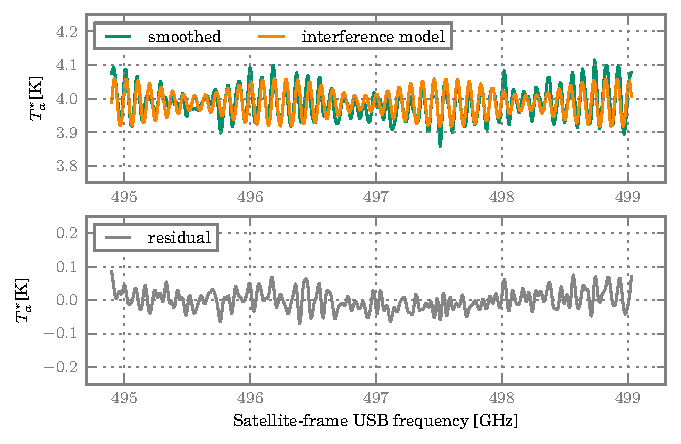
\includegraphics{mars_24_interf_smoothed_vs_interf}
    \caption{Same model applied to another spectrum}
    \label{fig:mars_24_interf_smoothed_vs_interf}
\end{figure}

The magnitude of the reflection coefficients given in~\cref{tab:mars_full_model} may appear surprising.
The calibration loads are supposed to be close to black bodies but the model predicts that the cold load reflects between 30 and \SI{70}{\percent} of the electric field intensity, which corresponds to a reflectivity in power between 10 and \SI{50}{\percent}.
In the next paragraphs we list hypotheses that can explain these surprising results.

The most obvious possible justification is that the data is noisy.
As shown in~\cref{fig:mars_filtered}, the thermal noise is almost as strong as the ripples that we are trying to measure.
We filter some of that noise by cutting the short-periods but that does not remove the contribution of that noise at the periods of our ripples.
The fitter treats that noise as if it were signal and converges toward somewhat incorrect values.

There is a degeneracy between the parameters: one equation for two variables.
Indeed, the behavior of a cavity depends on the product on the reflection coefficient of its two surfaces (see~\vref{eq:fabry_gain_r2_r3}).
For each coefficient of reflection of the mixer, we can find a coefficient of reflection of the hot and cold loads that reproduce the observed ripple: whenever one decreases the other increases to compensate with the same result.
To remove this degeneracy, we need more equations, which means more cavities.
If the LO--mixer cavity were less lossy, it would produce its own ripples and introduce one new equation to the problem, but it would also introduce one additional variable: the reflection coefficient of the LO itself.
This may still help: the load and the LO would form their own cavity (after reflection on the mixer).
With three parameters in three cavities, the degeneracy should disappear.

\begin{figure}
    \centering
    \input{hbb.pdf_tex}
    \caption{Photograph of the hot calibration load of HIFI.}
    \label{fig:hbb_photo}
\end{figure}
The model for the loads may be lacking.
We model the loads as a single plane surface because the Direct Fourier Transform of the HIFI data does not show any evidence of something mode complicated.
It may be the case, though, that the loads need to be modeled with two surfaces instead of one.
The hot load of HIFI is shown in~\cref{fig:hbb_photo}.
It is a wedge-shaped hole coated in an absorbent material.
Although the entire beam is supposed to couple to the wedge-shaped aperture, part of it may couple to the flat surface around it, especially in Band~1 where the beam is the widest.
A better model of the hot load may require two surfaces: one for the aperture and one for its surrounding.
Surprisingly high or low reflection coefficients may result from an inadequate model of the loads.

With more data we could constrain these parameters better and refine the model.
However, even in its current simple state and despite a low signal-to-noise ratio,
the qualitative predictions of the model seem satisfactory.





%#############################################################################
\FloatBarrier



\section{Conclusion}
A physically-based model of the optics of a coherent detector can predict the effects of interferences on the bandpass of that detector.

We created a physically-based model of the optics of HIFI Band~1 and compared its predictions to an actual HIFI observation of the planet Mars.
Despite the low signal-to-noise ratio and a lack of constraints on some parameters of the model, we reproduced the ripples seen on the continuum of the spectrum of Mars.
The amplitudes, frequency and phase of the modeled ripples are very close to the real ones.
Even if we could not constrain our model well enough to achieve a quantitative match in that specific case,
we consider that this is a successful proof of concept for our modeling technique.

We encourage instrument designers to allocate some time to measure the complex reflection coefficients of their optical components for different LO frequencies.
Matching the physically-based model to the real data would allow to correct the calibration by properly taking into account the ripples caused by the interferences in the optics.
%#############################################################################
%\clearpage
%\printbibliography[heading=subbibliography]
%\end{refsection}
